\section{Uveďte, jaké rušivé vlivy mohou působit na přenos}
\begin{itemize}
    \item \textbf{Šum} - náhodné změny fyzikální veličiny, které nepříznivě ovlivňují přenášený signál.
    \item \textbf{Rušení} - nepříznivé ovlivnění přenášeného signálu jiným elektrickým systémem.
    \item \textbf{Hluk} - Jde o všechny dynamické vlivy kanálu, které působí nepříznivě na přednášený signál
    \item \textbf{Šum} a rušení jsou podmnožinou obecného termínu hluk
    \item Významné rušivé jevy
    \begin{itemize}
        \item Jde o takové ručivé jevy, které mají náhodný charakter a velkou výkonovou  úroveň - impulsivní hluk, krátkodobý pokles úrovně signálu a krátkodobá změna fáze
        \item \textbf{Impulsní hluk} - Nejnebezpečnější.
        Má charakter krátkých vysokofrekvenčních kmitů o značné amplitudě, které se střídají s delšími bezhlukovými intervaly. Nebezpečí spočívá v relativně velké výkonové úrovny ve vztahu k přenášenému signálu a náhodnosti jeho charakteru.
    \end{itemize}
\end{itemize}

\section{Uveďte, proč je impulsní hluk považován za nejnebezpečnější}
viz. přechozí otázka

\section{Uveďte a popiště model vzniku chyb}
Zpráva je přenášena nejčastěji jako posloupnost dvou signálových prvků, kterým jsou přiřazeny hodnoty 0,1.
Chyby se projevují v posloupnosti dvoustavových signálových prvků jako inverze hodinty signálového prvku, tj. 0->1, 1->0.

Rušení se projeví inverzí hodnot určitých prvků, což můžeme modelovat pomocí sčítačky modulo 2

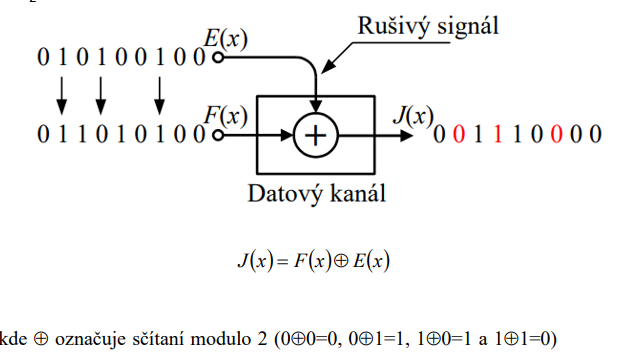
\includegraphics[]{images/ručení.png}
\begin{itemize}
    \item E(x) je chybová posloupnost - její strukturu zjišťujeme jako rozdíl F(x) a J(x).
    \item F(x) - posloupnost nul a jedniček přivedena na vstup datového kanálu.
    \item J(x) - posloupnost jedniček a nul na výstupu
    \item Je li přenost bezchybný, pak F(x) = J(x) a E(x) je posloupnost 0.
    \item K zápisu F(x),E(x) a J(x) se využívá mnohočlenů
\end{itemize}
\section{Vysvětlete pojmy: nezávislé chyby, shluky chyb, bitová chybovost, bloková chybovost}
\textbf{Nezávislé chyby} - Jejich rozložení je v přijaté zprávě relativně rovnoměrné.
Má tedy váznam hledat různé statistické odchylky
\begin{itemize}
    \item \textbf{Jednoduchá chyba} - Vyjadřuje skutečnost, že v signálu o \emph{n} prvků je pouze jeden prvek chybný
    \item \textbf{Vícenásobná chyba} - Vyjadřuje skutečnost, že v posloupnosti \emph{n} signálových prvlů se vyskytuje několik nezávislých chyb
\end{itemize}

Shluky chyb jsou takové úseky chybně přenesených prvkům ve kterých relativní četnost chybně přenesených prvků výrazně převyšuje četnost chybných prvků ve zbytku zprávy.
Počet chybných prvků ve shluku vyjadřujeme pomocí hustoty chyb shluku v \%

\section{Co udává kódový poměr a kódový zisk. Co je Shannonův limit}
Kódový poměr - ???

\textbf{Kódový zisk} - protichybové kódování umožňuje snížit odstup SNR(odstup signál-šum) při udržení stejné chybovosti.
Poměr potřebného SNR$_{NEKOD}$ ku SNR$_{KOD}$ s kódováním se označuje jako kódový zisk. 
Jeho jednotkou je [dB].

\textbf{Shannonův limit} říka, že pro daný kódový poměr R musí být dosažena určita minimální hodnota SNR.
Tato minimální hodnota se nazývy Shannonův limit, je uvedena v [dB].

\section{Uveďte základní dva typy protichybových kódových systémů, jejich výhody a nevýhody}
\begin{itemize}
    \item \textbf{Zabezpeční pomocí opravných protichybových kódů:} Metoda vyžaduje pouze jednosměrný přenos dat.
    Vložená nadbytečnost ve vysílači umožňuje chyby v přijímači opravit
    \item \textbf{Zabezpečení pomocí detekčních protichybových kódů s opakováním chybného přenosu - Automatic Repeat Request: }každá přenesená sekvence dat je potrvzována přijímačem.
    Při chybě je chybná sekvence zopakována.
    Existuje několik metod ARQ - Stop-and-Wait, go-back, selective
\end{itemize}
\section{Vysvětlete rozdíl mezi zabezpečením blokovým a stromovým kódem}
\begin{itemize}
    \item \textbf{Blokové kódy:} Zabezpečovací proces je realizován pouze v rámci jediného bloku dat, který vznikl rozdělením datového toku do úseků o definovaném počtu k-signálových prvků.
    \item \textbf{Stromové kódy: }Zabezpečovací proces je realizován nejen na základě jediného bloku dat, ale využívá se k němu navíc m-1 předchozích k-prvkových bloků dat.
    Vzniklá závislost zabezpečovací sekvence je dalším zapezpečovacím prvkem.
\end{itemize}

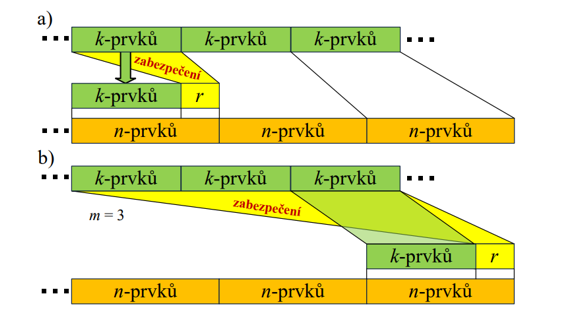
\includegraphics[]{images/zabezpečování.png}

\section{Co udává hammingova vzdálenost a váha? Vyvětlete využití}

\begin{itemize}
    \item \textbf{Hammingova vzdálenost (d):} Udává počet míst, ve kterých se dvě kombinace prvků ve sledovaném úseku zprávy mezi sebou liší.
    

    
    \item \textbf{Hammingova váha (w):} Udává počet nenulových prvků v kódovém slove.
    Minimální Hammingova váha je nejmenší váha mezi všemi kódovými slovy kromě slova s nulovými prvky.
    
    \item Využívá se v protichybovém kódování, kde uměleje snižujeme $d_{min}$ tak, že k signálovým prvkům nezabezpečené zprávy přidáváme zabezpečovací prvky podle pravidel definujicích použitý protichybový kód.
    Jiná možnost dosažení d$_{min}$ spočívá ve výběru takových posloupností signálových prvků ze všech možných posloupností signálových prvků délky n rozdělí na užívané posloupnosti, které tvoří protichybový kód a neužívané posloupnosti.  Při tomto způsobu tvorby kódu můžeme rozlišit původní nezabezpečené prvky a zebezpečovací prvky.
\end{itemize}
\section{Vysvětlete princip zabezpečení zpráv proti chybám a a jeho vysvětlení}
???

\section{Co určuje Plotkinova hranice}
Používá se k určení minimální potřebné délky kódového slova k dosažení požadované korekční či detekční schopnosti kódu.